\documentclass[a4paper,12pt,twoside]{article}
\usepackage[left=3cm,right=3cm,top=2cm,bottom=3cm]{geometry}
%\usepackage[square,authoryear,sort]{natbib}
\usepackage{url}
\usepackage{xcolor}
\usepackage{graphicx}
\usepackage{subcaption}

\makeatletter
\def\@makesectionhead#1{%
  \vspace*{50\p@}%
  {\parindent \z@ \raggedright \normalfont
    \interlinepenalty\@M
    \Huge\bfseries  \thesection.\quad #1\par\nobreak
    \vskip 40\p@
  }}
\makeatother

\makeatletter
\newcommand*{\toccontents}{\@starttoc{toc}}
\makeatother

\newtheorem{hypothesis}{Hypothesis}

\newtheorem{rquestion}{Research Question}


\let\endtitlepage\relax
\begin{document}

\title{\LARGE {\bf Semantic Modelling of Network Traffic for Anomaly Detection}\\
PhD 2\textsuperscript{nd} Year Progress Report
 \vspace*{-5mm}
}
\author{Henry Clausen}
%\date{October 2008}

\maketitle



\toccontents
%\begin{abstract}
%Text
%\end{abstract}


\section{Introduction}

\subsection{Central Research questions}

\begin{rquestion}\ \\ 
How well-structured is the space of contextual behaviours observed in the traffic of a machine or a network? How much does noise or input variation blur the observable contextual differences between clearly distinct actions?

%\begin{enumerate}
%\item How can we scientifically quantify closeness between individual actions, and does it translate into the similarity of corresponding traffic structures? 
%\end{enumerate}
\end{rquestion}



\begin{rquestion}\ \\
To what degree can contextual structure in network traffic be captured in a model from a training dataset, and how can we achieve this? How can a model adapt to changes of normal contextual structures?
%\begin{enumerate}
%\item Which parts of network traffic both contain important information and can be represented by a model?
%\item Can be combine models that act at different traffic levels to enhance the amount of context given by the data? 
%\item Can we efficiently disentangle overlaying network flows to isolate otherwise distorted flow groups corresponding to similar actions? 
%\item What is an efficient and realistic way to incorporate other data sources into the modelling procedure? How can this input enhance the learning process and the representation detail of a traffic model? 
%\item How can a model adapt to changes of normal contextual structures?
%\end{enumerate}
\end{rquestion}

\begin{rquestion}\ \\
What is a meaningful representation of traffic structures? What requirements must a labelled traffic generation framework fulfill to provide realistic data?
%\begin{enumerate}
%\item What requirements must a labelled traffic generation framework fulfill to provide realistic data?
%\item Can we evaluate the traffic representation of a model through its ability to identify contextual closeness between traffic instances correctly?
%\item How can we quantify the capability of a given traffic model to identify new computational actions on a machine?
%\end{enumerate}
\end{rquestion}


\begin{rquestion}\ \\
What will a contextual model be able to prevent? 
%\begin{enumerate}
%\item What kind of attacks will necessarily show contextual anomalies, and which will not?
%\item Can an adversary adapt his attacks to avoid detection? How can we prevent this?
%\end{enumerate}
\end{rquestion}

\subsection{Motivation}

Newer models clearly leverage microstructures

However, traffic opaque 

...

\subsubsection{Relevance}

\subsection{Thesis overview}

\subsection{Background}

\subsection{Network traffic}\label{traffic}



Computers in a network mostly communicate with each other by sending \textit{network packets} to each other, in which the transmitted information is encapsulated. Each network packet is split into the control information, also called packet header, and the user information, called payload. The packet header contains the necessary information for the correct transmission of the packet, including the transmission protocol layer (such as TCP, UDP, or ICMP), and the source and destination IP addresses and network ports\footnote{A network port is a number that identifies which service or application is responsible for the processing of incoming packets.}. It furthermore contains error-checking fields suchs as the size of the packet and a checksum over the payload, and protocol-specific fields. 


\begin{figure}[h!]
\centering
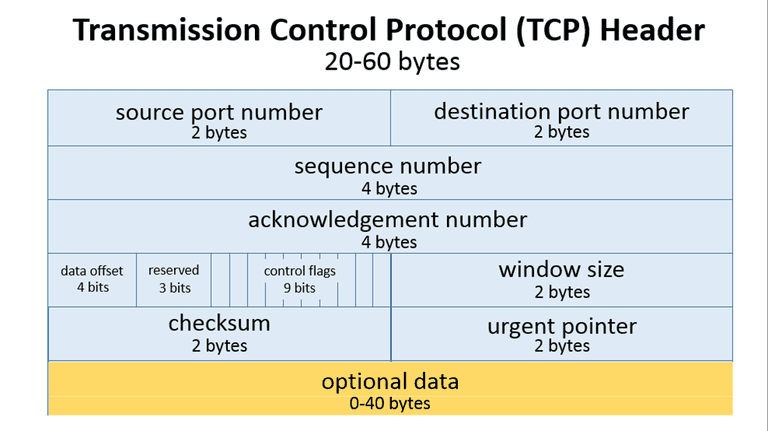
\includegraphics[scale=0.4]{images/tcp_header.png}
\caption{Typical format of a TCP packet. Source:\scriptsize{ https://www.lifewire.com/tcp-headers-and-udp-headers-explained-817970}\normalsize}
\end{figure}


The payload of a packet is in general the data that is carried on behalf of an application. It can be of variable length, however, it cannot exceed the maximum packet length set by the network protocol. In contrast to the packet header, the payload can be encrypted, a technique that makes it unreadable to any third parties and that is becoming increasingly common in modern computer networks. 


While traversing between to parties, a network packet can pass multiple connecting devices which direct the packet in the right direction. Any device in the immediate circuit traversed by a packet can capture and store it. In a monitoring setting, packets are usually captured by network routers and stored in the widespread \textit{pcap} format. In case of space shortage or privacy concerns, the payload of a packet can be dropped in the saving process.


Another more structured way of capturing network traffic is based on connection summaries, or \textbf{network flows}. RFC 3697 \cite{brownlee1999traffic} defines a network flow as a sequence of packets that share the same source and destination IP address, IP protocol, and for TCP and UDP connections the same source and destination port. A network flow is usually saved containing these informations along with the start and duration of the connection and the number of packets and bytes transferred in the connection.


\begin{figure}[h!]
\scriptsize
\centering
\begin{verbatim}
 Date flow start        Duration Proto  Src IP Addr:Port      Dst IP Addr:Port   Packets  Bytes Flows
 2010-09-01 00:00:00.459   0.000 UDP    127.0.0.1:24920   ->  192.168.0.1:22126      1     46     1
 2010-09-01 00:00:00.363   0.000 UDP    192.168.0.1:22126 ->  127.0.0.1:24920        1     80     1
\end{verbatim}
\normalsize
\caption{A typical network flow output}
\end{figure}


Raw packets grant full information about the connection, but take a lot of space when stored, whereas network flows give a more structured and lightweight overview over the traffic in a network. Both data formats are used widely by NIDSs.

\subsection{Intrusion detection}

Sophisticated data breaches affect hundreds of million customers and inflict tremendous financial, reputational, and logistic damage. One reason for the recent rise of cyber crime is the increased use of advanced techniques for the attack of specific targets. Attackers use customised social engineering and custom-built malware that penetrate defensive barriers and potentially stay undetected in an infected system for an extended period of time. 

Cyber-security relies on a range of defensive techniques, including sophisticated intrusion detection systems and firewalls that try to detect and prevent attacks against software subsystems. Malicious software still remains the biggest threat to computer users, and its detection is of utmost importance. 

The field of intrusion detection is concerned with the development of methods and tools that identify and locate possible intrusions in a computer network. An \textit{intrusion detection system} (IDS) is typically a device or software application that detects malicious activity or policy violations in an automated way by scanning incoming data collected from one or more sources for patterns that a model or a set of rules classifies as potentially malicious.

Intrusion detection is a well researched area, with the first IDSs emerging in the late 1980's. Intrusion detection today comprises a variety of research areas in terms of different types of data sources, system architectures, detection sope, and so forth. Denning \cite{denning1987intrusion} in 1987 established the notion of two different types IDS implementations: a) host-based and b) network-based. 
\textit{Host-based intrusion detection systems} (HIDS) monitor each host in a network individually, and rely on local data streams such as application logs or raw operating system calls as  data source. \textit{Network-based intrusion detection} refers to the detection of malicious traffic in a network of computers and uses network traffic captures as a data source. In this PhD project, I will mainly focus on network traffic as a data source due its universal nature, its resilience against modification, and my previous experience in the field. However, I will also investigate the possibility of relating both types of traffic. For more details on IDS implementations, I refer the reader to my more detailed literature review. 


Current detection methods are predominantly based on the analysis of previously identified attack signatures, which provides great reliability and low false alert rates. However, these methods are dependent on an updated attack signature database and provide no protection against previously unseen attacks. With attackers having access to more resources than ever, custom built malware is becoming more common to circumvent signature-based detection. 

Another approach that has recently gained traction in commercial deployment is based on detecting malware and other undesired activity as anomalous behaviour when compared to benign computer activity. In this approach, known as \textbf{network anomaly detection} after Denning \cite{denning1987intrusion}, models must quantify the behaviour of normal network behaviour to be independent of a narrowly defined notion of malicious activity.

\subsection{Intrusion Detection Systems}

The field of intrusion detection is concerned with the development of methods and tools that identify and locate possible intrusions in a computer network. An \textit{intrusion detection system} (IDS) is typically a device or software application that detects malicious activity or policy violations in an automated way by scanning incoming data collected from one or more sources for patterns that a model or a set of rules classifies as malicious.

Intrusion detection is a well researched area, with the first IDSs emerging in the late 1980's. Intrusion detection today comprises a variety of research areas in terms of different types of data sources, system architectures, detection sope, and so forth. Figure \ref{graph} provides a broad yet uncomplete overview of these different areas. 

\subsubsection*{Implementation}

Denning \cite{denning1987intrusion} in 1987 established the notion of two different types IDS implementations: a) host-based and b) network-based. 
\textit{Host-based intrusion detection systems} (HIDS) monitor each host in a network individually, and rely on local data streams such as application logs or raw operating system calls as  data source. A relatively new form of host-based data sources are biometrik user data such as keystrokes or eye movement, please see \cite{peng_user_2016} for more information.

\textit{Network-based intrusion detection} refers to the detection of malicious traffic in a network of computers. A network intrusion detection system (NIDS) monitors network traffic within in a network and/or between the network and external hosts for malicious activity or policy violations. Network traffic data can take different forms, a more detailled explanation will be provided in Section \ref{traffic}.

\begin{figure}\label{graph}
\centering
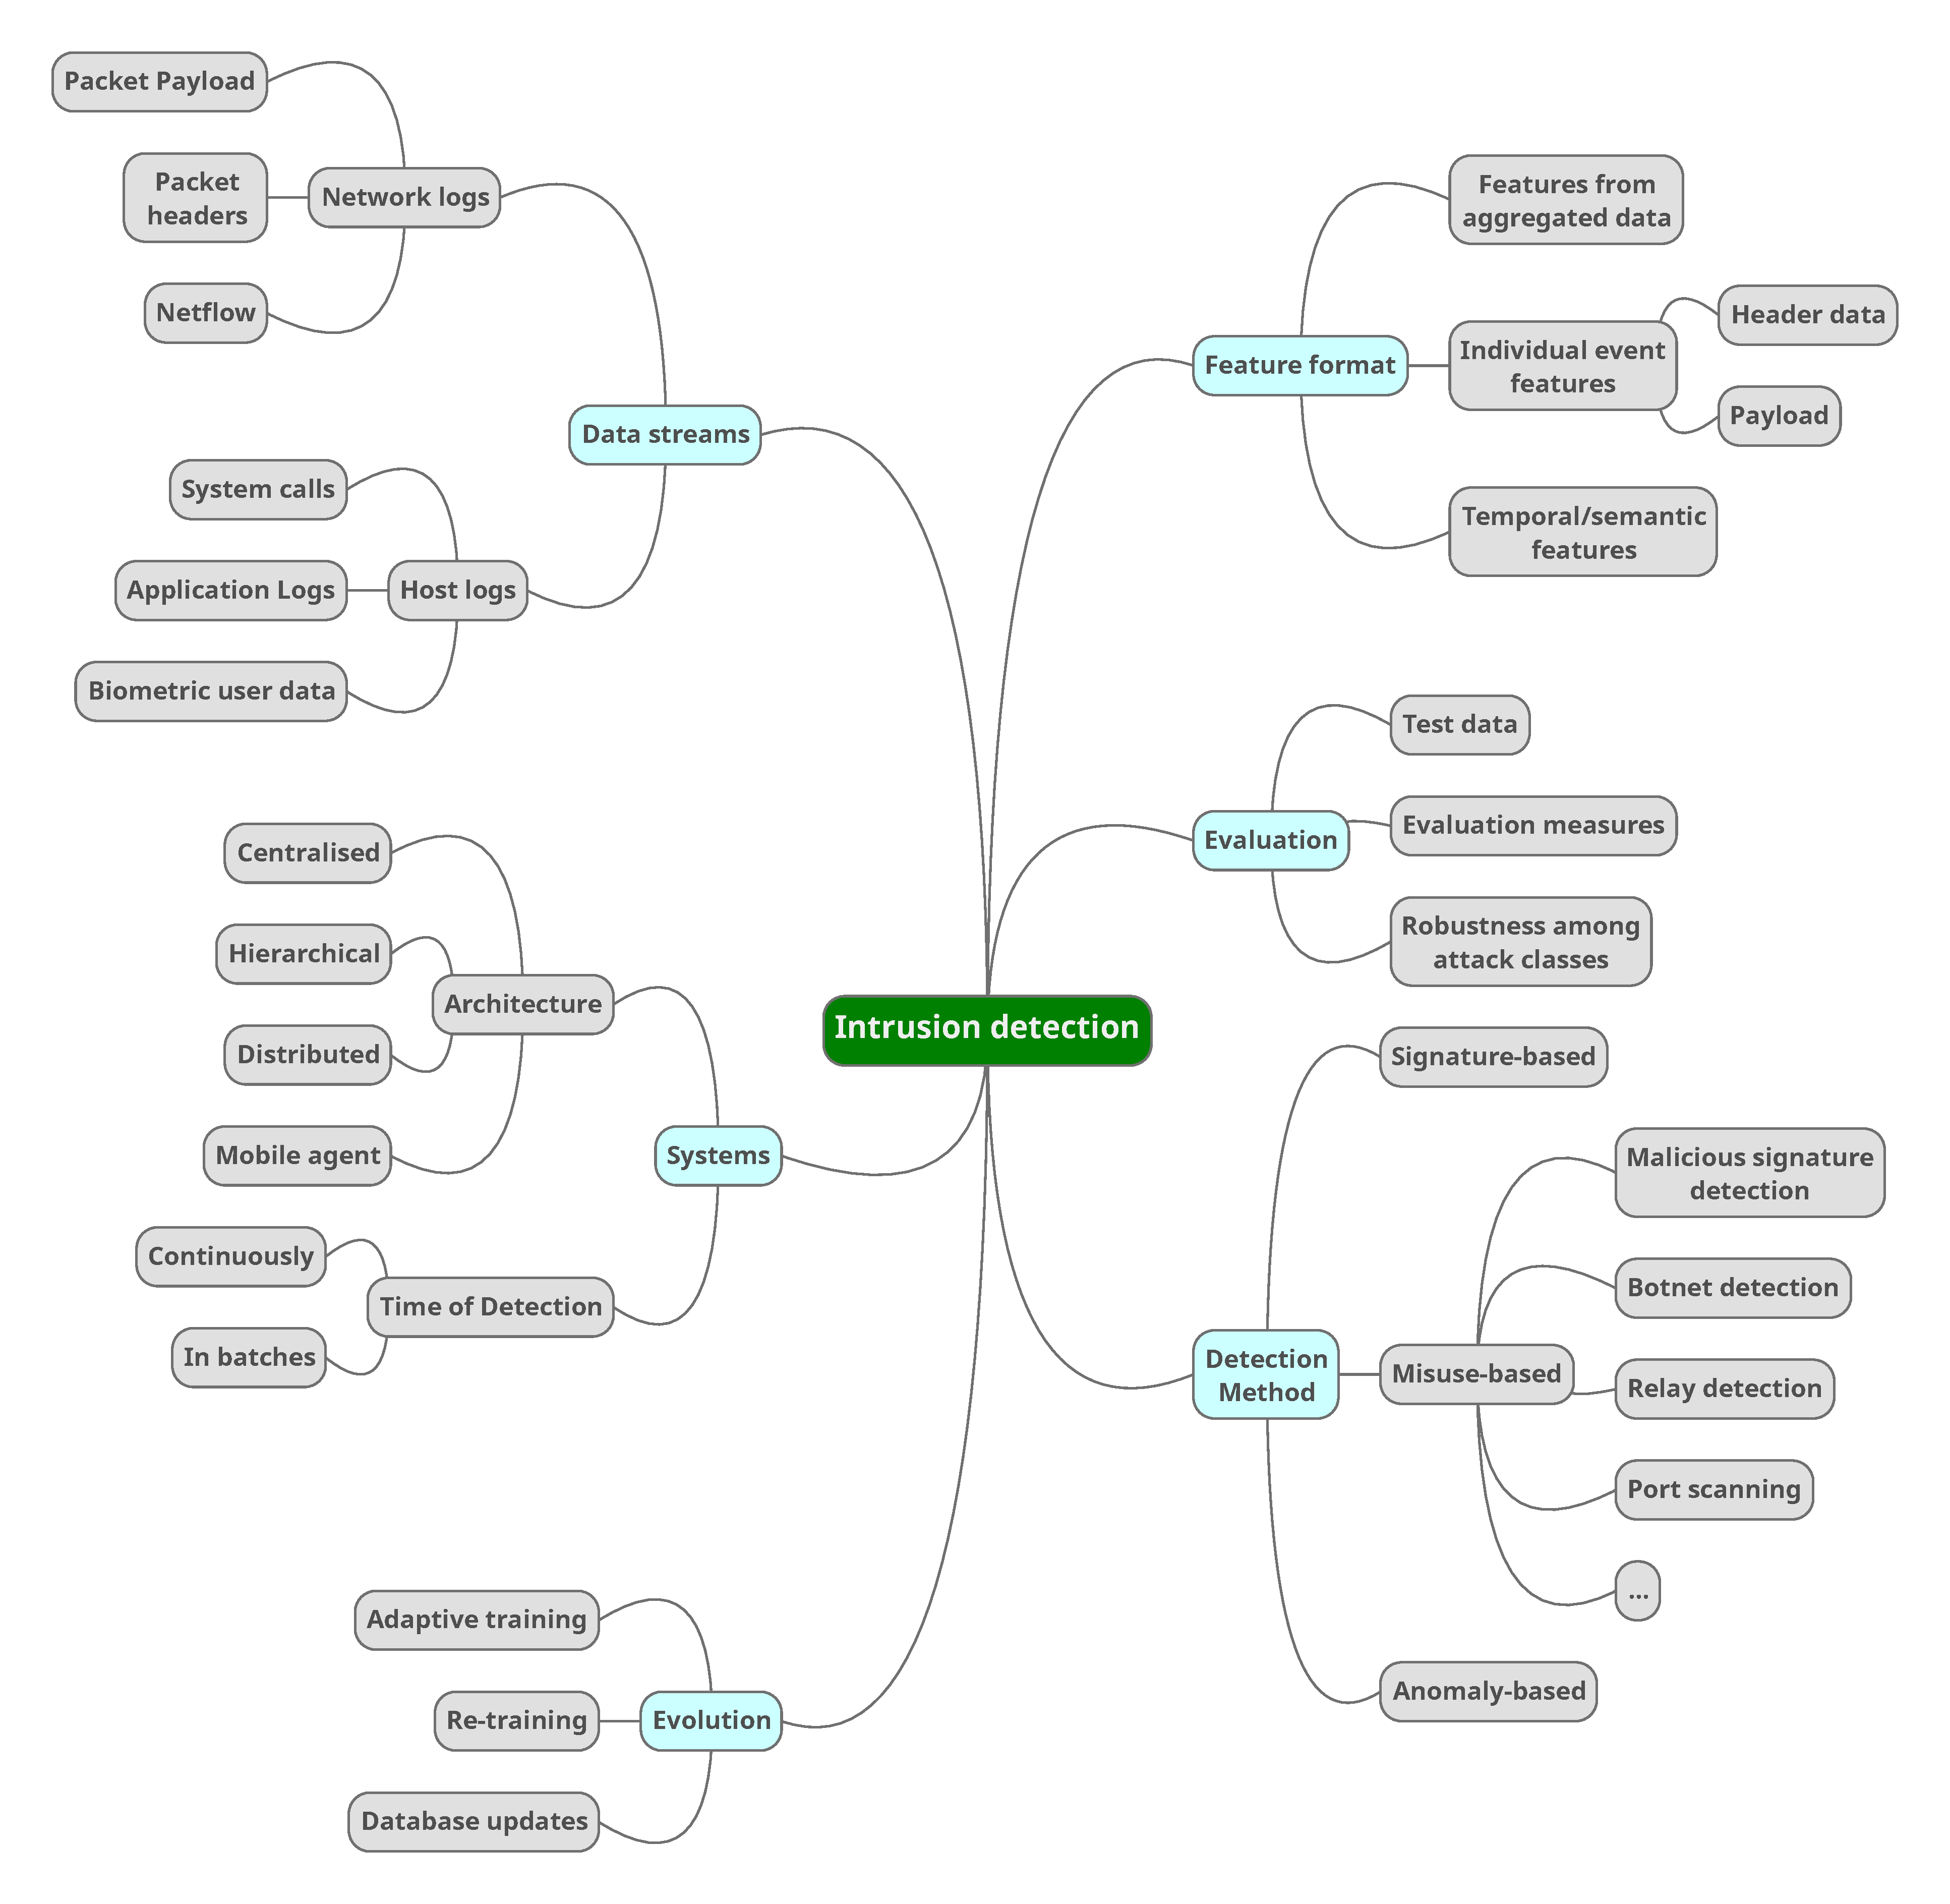
\includegraphics[scale=0.25]{images/Graphic2.pdf}
\caption{A broad overview over different aspects in an IDS}
\end{figure}

Host-based systems have the advantage of working with high quality data that   are   typically   very   informative \cite{lazarevic2005intrusion}. NIDS have the advantage of being plattform independent and more resiliant to attacks as detection of an infection is not done on the infected system. In this review, I will focus on work done in the area of network intrusion detection.


\subsubsection*{Detection methods}

Detection methods are the core of an IDS, and are therefore the most important design choice. Traditionally, two broad types of detection approaches are identified: a) Misuse detection and b) anomaly detection. 

Misuse detection aims at detecting a particular and well known reoccurring characteristic or pattern of a malicious behaviour. Two simple examples of such a characteristic are the large number of SYN packets sent by a host in a DoS attack, and the synchronised connection of many hosts to one server in a botnet. In misuse detection, abnormal or malicious behaviour is therefore defined first before developing a model to distinguish the defined behaviour from other traffic.

In contrast, anomaly detection aims at building a model of normal system behaviour that is accurate enough to spot any malicious behaviour as traffic that deviates from the estimated model. Anomaly detection is principally more difficult than misuse detection since the traffic model has to incorporate potentially very heterogenuous traffic behaviours. However, it is generally acknowledged that anomaly detectionhas is more suitable to detect new and previously unseen malicious behaviour as it makes no definite assumptions on the anomalous behaviour. Misuse detection is robust against evolution of malware as long as defined malicious behaviours do not change.

In reality, anomaly and misuse detection are not necessarily mutually exclusive, and there is a fluent passage between the two. This is because many anomaly detection approaches choose a particular set of features to be modelled with a particular threat in mind. For instance, models for the number of connections of a machine are naturally suitable for detecting DoS attacks, port scans, or Worm attacks. 

As misuse detection detection methods are aimed at detecting very specific behaviour, they usually only detect one type of malicious traffic. Areas that have been researched particularly well include botnet C\&C channel detection, DoS attack detection, and port scan detection. Areas that lack a comprehensive body of research are different types of R2L and U2R attacks. These are also currently the least   detected   attack   classes \cite{nisioti2018intrusion}.

\subsection{Anomaly detection}

Anomaly detection refers to the problem of identifying data instances that have significantly different properties than previously observed ``normal data instances. Anomaly detection has its origins in statistical research where normal data instances are assumed to be generated as random variables by a probability distribution $P_\textit{N}(X)$. New data is then identified as anomalous if its properties correspond to regions with vanishing likelihood, i.e. this particular data instance is highly unlikely to be generated by $P_\textit{N}(X)$. Usually, the hard part in anomaly detection is to use observed data efficiently to build an estimated distribution $\hat{P}_\textit{N}(X)$ that resembles $P_\textit{N}(X)$ closely to identify anomalous events while asigning normal instances a non-vanishing likelihood. A variety of techniques exist to achieve this assuming comparably simple generating distributions. However, distributions for many interesting types of normal data can be complex and changing over time, and individual data points can have intricate interdependencies. 
\begin{figure}
\centering
\begin{subfigure}[b]{0.45\textwidth}
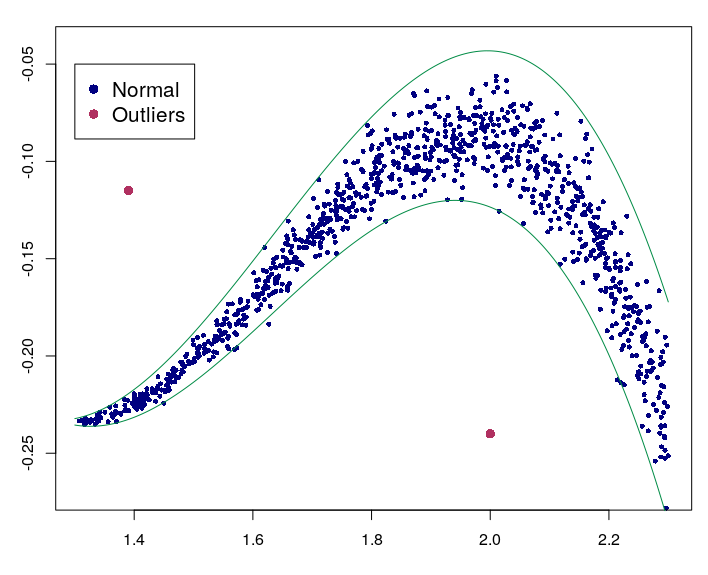
\includegraphics[width=\textwidth]{images/outlier_mine.png}
\caption{}
\end{subfigure}
\begin{subfigure}[b]{0.45\textwidth}
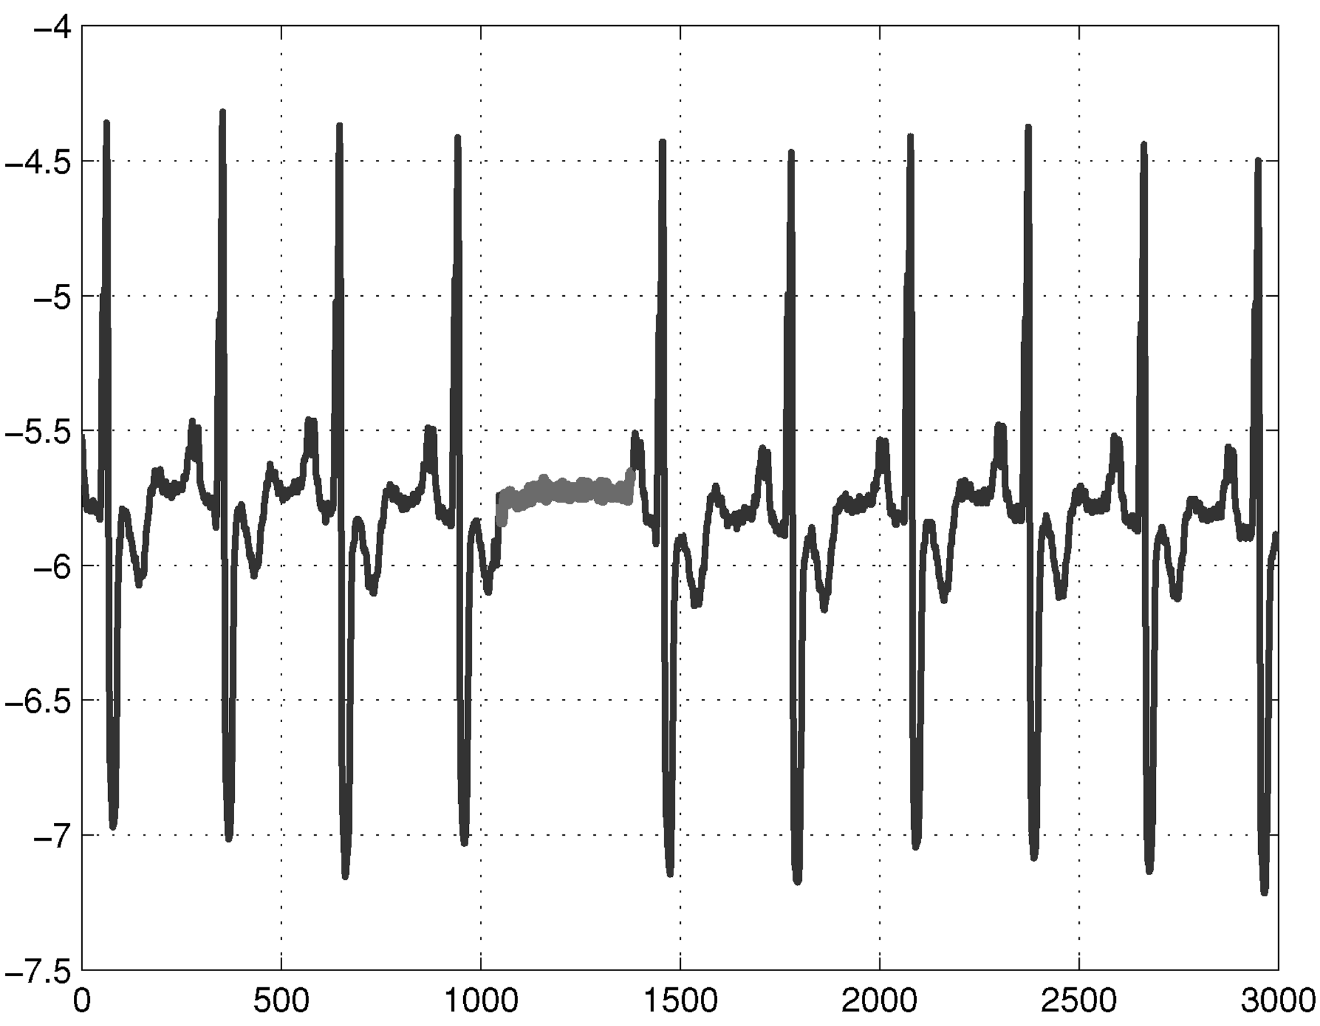
\includegraphics[width=\textwidth]{images/Atrial_Premature_Contraction.png}
\caption{}
\end{subfigure}
\caption{The left plot (a) depicts simple anomalies that deviate in distance from regular data. The right plot (b) shows a contextual anomaly where a group of data instances do not follow a repeating timely behaviour with respect to all other data points (corresponding to an \textit{Atrial Premature Contraction}, taken from \cite{chandola_anomaly_2009})}\label{graph}
\end{figure}

Anomaly detection has found wide application in areas where stability of  critical systems or detection of their abuse is crucial. Examples of these include engine-fault detection in wind-turbines and fraud detection for credit cards. The assumption here is that the modelled system, such as the sensor-data stream of an engine or the buying behaviour of a customer, remains stable and generates consistent data. Detected anomalies in new observations then indicate a potential fault or abuse in this system. Obviously, it is not inherently clear that every abuse or fault generates data that differs from normal data. Therefore, it is important to choose data sources that are able to reflect the unique nature of a particular system.

\subsubsection{Anomaly detection and NIDS}

Anomaly detection has been applied to network security since the late 90's to assist IDSs. The behaviours of network computers are usually captured in the form of events logs such as network packets or flows, system calls, etc. The basic approach is to use collected training logs to infer a model of trustworthy activity, and then compare newly observed behaviour against this model.  To prevent any anomaly model from learning malicious behaviour as normal, the used training data has to be free of any attacks\footnote{Again, the assumption is that unauthorized and malicious activity will correspond to behaviour that differs from trustworthy one.}. 

As an example, an anomally large network flow involving an unusual pair of network computers could indicate that a hacked computer is extracting or sending out sensitive data to an unauthorized destination. An anomaly detection model does not make any assumptions about attack behaviour, but instead marks all deviations from the learned normal behaviour as potentially malicious. It is therefore better suited to find novel and unseen attacks. However, features mined from the data have to be able to reflect normal behaviour in a way that malicious traffic will look different in order to be detectable, which is not trivial. Furthermore, normal instances that only occur rarely or are diffuse will potentially also be flagged as potentially malicious, making an anomaly-based IDS prone to high false alert rates.


\section{Controlling traffic and corresponding microstructures}



\section{How traffic models are susceptible to microstructures}

Include some of the findings from the stepping stone paper here:

\begin{itemize}
\item How models such as DeepCorr are set up to capture sequential dependencies
\item How they are sucsceptible to chaff, long rtts, etc.
\end{itemize}

\subsection{Models that rely explicitely on microstructure modelling}
Basically traffic classifiers


%\section{Application to intrusion-detection}


\section{Capturing traffic microstructures on a flow-level with a bidirectional LSTM}

\section{Capturing traffic microstructures on a packet-level with a LSTM-encoder}



\section{Thesis plan}

In the light of the problems described in Section \ref{Sec:Problems} that we encountered in the field of anomaly-based intrusion detection, I believe that the scope of this PhD-project has to be altered slightly. As there will not be enough material directly concerning anomaly detection, the formulation of building anomaly-detection models describing software behaviour should be relaxed to general applications of ML (not just anomaly detection) in specific areas related to software defined behaviour. 
The overall unifying theme of this PhD so far has been centered around small-scale traffic structures generated by software-defined computer interactions and applications of ML language models to it, in other words \textbf{Modelling computer interactions as a language}.
This could be based of the reoccurring use of traffic (and potentially system/program logs) generation for machine learning. The generated traffic could then be verified as valuable by the implemented intrusion detection applications.

All applications implemented so far except for the flow-level model are driven (in part) by our traffic generation:
\begin{itemize}
\item Flow-level LSTM model

\item stepping stone detection
\item traffic relay
\item LSTM encoder
\item QUIC anomaly detection
\end{itemize}

Overall, all these applications except for the traffic relay detection are concerned with software-defined fine-grained structures. Below, I outline the different chapters that I believe should be included in my thesis:

\begin{enumerate}


\item Introduction and related work

This chapter could largely draw from the existing introduction in the research proposal as well as the extensive literature survey I conducted. Updates on the scope as well as recent developments in related work would have to be added. %This should take less then three weeks.

\item Background: Anomaly detection and challenges in security

This chapter outlines the motivation to use anomaly-based detection models instead of classification-based ones. It furthermore highlights why anomaly detection is more difficult in security than in other areas, and what currently prevents it from being deployed outside of academia.

\item Background: Language models and their application to security

This chapter briefly outlines different techniques used in language modelling,  and how they can be used to build data representation useful for anomaly-detection. It also discusses previous applications of language models in security.

\item Data sources, datasets, and data generation with realistic small scale structures

This chapter will draw largely on the work conducted for the DetGen traffic generation framework.

\item Computer communication structures and the effect of malicious behaviour on them

This chapter will describe the different structures that the different layers of software-defined communication can have on the collected data. These descriptions and their corroboration can be taken from work in each of the projects described above. Furthermore, this chapter will describe how attacks can alter these structures due to the distinct approach they are taking, and why it is worth building models that focus on small-scale traffic structures.

\item Traffic as a language and detection models

This chapter will describe how network traffic can be described by a language model, and how to construct anomaly-based models from it. The chapter will then proceed to describe the different approaches I worked on and their respective results:

\begin{enumerate}

\item Flow-based modelling

\item Connection setup model

\item Traffic relating to process initialisations in the QUIC protocol

\item Detecting similarity in computer connections


\end{enumerate}

\item Conclusions

\end{enumerate}


%\addcontentsline{toc}{section}{Bibliography}
\bibliographystyle{abbrv}
\bibliography{refs}

\end{document}